\documentclass{article}

\usepackage[dutch]{babel}
\usepackage[margin=3cm]{geometry}
\usepackage{graphicx}

\graphicspath{
    {img/}
}

\newcommand{\bold}[1]{\textbf{#1}}

\begin{document}

\begin{titlepage}
    \author{Tuur Vanhoutte}
    \title{Sensors \& Interfacing}
\end{titlepage}

\pagenumbering{gobble}
\maketitle
\newpage
\tableofcontents
\newpage

\pagenumbering{arabic}

\section {Communicatie}
\subsection{Datacommunicatie in IoT}
3 lagen:
\begin{enumerate}
    \item Application Layer
    \item Fog layer
    \item IoT Device Layer
\end{enumerate}

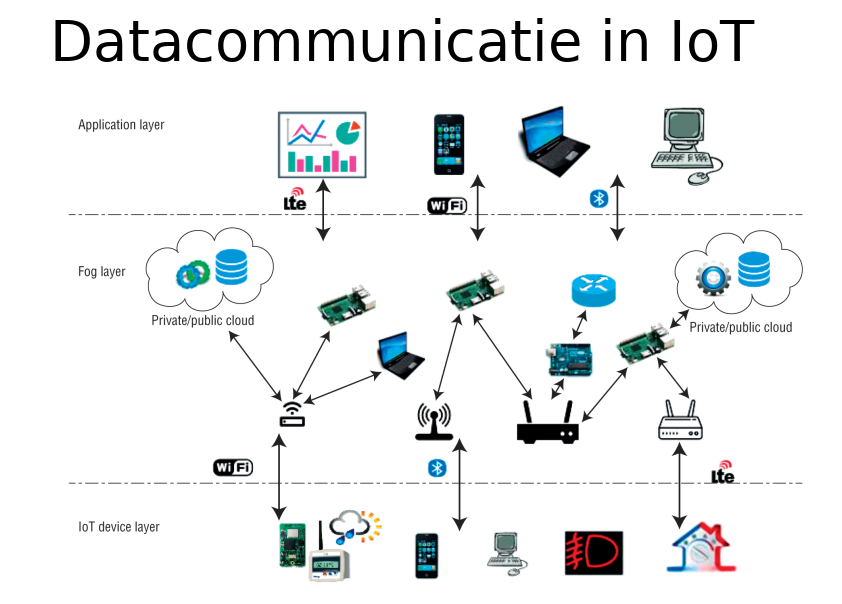
\includegraphics[width=\textwidth]{Screenshot_20200210_120010.png}

\subsection{Data}
\begin{itemize}
    \item "Pre-informatie"
    \item Gegevens waaruit informatie kan worden gewonnen
    \item Stelt een bepaalde toestand voor
\end{itemize}

\subsection{Communicatie}
Overbrengen van informatie tussen deelnemers
\begin{itemize}
    \item Boodschap
    \item Signaal
    \item Medium
\end{itemize}

\subsubsection{Communicatieafspraken}
\begin{itemize}
    \item Coderen van informatie (encoding)
    \item Voorbeeld:
        \item morse-code
        \item Ascii-codering
        \begin{itemize}
            \item Codering voor alle gebruikte symbolen in symbolen
            \item Codering in 7 of 8 bit
            \item 1 byte = 1 teken
        \end{itemize}
        \item \dots
\end{itemize}

\subsubsection{Encoding/Decoding}
\begin{enumerate}
    \item Codifying
    \item Sending the message
    \item Decodifying
\end{enumerate}

\subsubsection{Signalen}
\begin{itemize}
    \item Licht
    \item Geluid
    \item Elektriciteit
    \item \dots
\end{itemize}

\subsubsection{Communicatiemedia}
\begin{itemize}
    \item Twisted-Pair cable
    \item Coaxial cable
    \item Fiber-Optic cable
\end{itemize}

\subsubsection{Voorbeelden}
\begin{itemize}
    \item Welke codering?
    \item Wat is het signaal?
    \item Wat is het medium?
\end{itemize}

\subsubsection{Eigenschappen van media}
\begin{itemize}
    \item Vatbaarheid voor interferentie
    \item Overbrugbare afstand
    \item Praktisch
    \item Kostprijs
\end{itemize}

\subsubsection{Afspraken}
\begin{itemize}
    \item Protocol
    \item Standaarden
    \item IEEE
    \item EIA (NEDA/ECA)ECIA
\end{itemize}

\subsubsection{Standaardiseren van \dots}
\begin{itemize}
    \item Type media en zijn specificaties
    \item Het gebruikte signaal en zijn toleranties
    \item De elektrische interferentie
    \item De gebruikte codering
    \item Foutcorrectiecodes
    \item Protocol
    \item De gebruikte connector
    \item \dots
\end{itemize}

\end{document}
